%%%%%%%%%%%%%%%%%%%%%%%%%%%%%%%%%%%%%%%%%
% Beamer Presentation
% LaTeX Template
% Version 1.0 (10/11/12)
%
% This template has been downloaded from:
% http://www.LaTeXTemplates.com
%
% License:
% CC BY-NC-SA 3.0 (http://creativecommons.org/licenses/by-nc-sa/3.0/)
%
%%%%%%%%%%%%%%%%%%%%%%%%%%%%%%%%%%%%%%%%%

%----------------------------------------------------------------------------------------
%	PACKAGES AND THEMES
%----------------------------------------------------------------------------------------

\documentclass{beamer}
\usepackage[spanish]{babel}

\usepackage[T1]{fontenc}
\usepackage[utf8]{inputenc}

\usepackage[style=apa,backend=biber]{biblatex}
\DeclareLanguageMapping{spanish}{spanish-apa}
\bibliography{references}
\AtBeginBibliography{\scriptsize}

\usepackage{graphicx}
\usepackage[export]{adjustbox}
\graphicspath{{images/}{video/}}

% Para símbolos matemáticos
\usepackage{amsfonts}
\usepackage{amsmath}
\newcommand{\Mod}[1]{\ (\mathrm{mod}\ #1)}

% Símbolo de euro
\usepackage[gen]{eurosym}

% Para \url{}
\usepackage{hyperref}
\hypersetup{
  colorlinks=true,
  linkcolor=blue,
  filecolor=magenta,
  urlcolor=cyan,
}

\mode<presentation> {

% The Beamer class comes with a number of default slide themes
% which change the colors and layouts of slides. Below this is a list
% of all the themes, uncomment each in turn to see what they look like.

%\usetheme{default}
%\usetheme{AnnArbor}
%\usetheme{Antibes}
%\usetheme{Bergen}
%\usetheme{Berkeley}
%\usetheme{Berlin}
%\usetheme{Boadilla}
%\usetheme{CambridgeUS}
%\usetheme{Copenhagen}
%\usetheme{Darmstadt}
%\usetheme{Dresden}
%\usetheme{Frankfurt}
%\usetheme{Goettingen}
%\usetheme{Hannover}
%\usetheme{Ilmenau}
%\usetheme{JuanLesPins}
%\usetheme{Luebeck}
\usetheme{Madrid}
%\usetheme{Malmoe}
%\usetheme{Marburg}
%\usetheme{Montpellier}
%\usetheme{PaloAlto}
%\usetheme{Pittsburgh}
%\usetheme{Rochester}
%\usetheme{Singapore}
%\usetheme{Szeged}
%\usetheme{Warsaw}

% As well as themes, the Beamer class has a number of color themes
% for any slide theme. Uncomment each of these in turn to see how it
% changes the colors of your current slide theme.

%\usecolortheme{albatross}
%\usecolortheme{beaver}
%\usecolortheme{beetle}
%\usecolortheme{crane}
%\usecolortheme{dolphin}
%\usecolortheme{dove}
%\usecolortheme{fly}
%\usecolortheme{lily}
%\usecolortheme{orchid}
%\usecolortheme{rose}
%\usecolortheme{seagull}
%\usecolortheme{seahorse}
%\usecolortheme{whale}
%\usecolortheme{wolverine}

%\setbeamertemplate{footline} % To remove the footer line in all slides uncomment this line
\setbeamertemplate{footline}[page number] % To replace the footer line in all slides with a simple slide count uncomment this line

\setbeamertemplate{navigation symbols}{} % To remove the navigation symbols from the bottom of all slides uncomment this line
}

\usepackage{graphicx} % Allows including images
\usepackage{booktabs} % Allows the use of \toprule, \midrule and \bottomrule in tables
%\usepackage {tikz}
\usepackage{tkz-graph}
\GraphInit[vstyle = Shade]
\tikzset{
  LabelStyle/.style = { rectangle, rounded corners, draw,
                        minimum width = 2em, fill = yellow!50,
                        text = red, font = \bfseries },
  VertexStyle/.append style = { inner sep=5pt,
                                font = \normalsize\bfseries},
  EdgeStyle/.append style = {->, bend left} }
\usetikzlibrary {positioning}
%\usepackage {xcolor}
\definecolor {processblue}{cmyk}{0.96,0,0,0}
%----------------------------------------------------------------------------------------
%	TITLE PAGE
%----------------------------------------------------------------------------------------

\title[Short title]{Estudio de viabilidad del uso de librerías de criptografía homomórfica en procesos reales} % The short title appears at the bottom of every slide, the full title is only on the title page

\author{\textbf{Autor}: Javier Junquera Sánchez \\ \textbf{Tutor}: Alfonso Muñoz Muñoz} % Your name
\institute[UEM] % Your institution as it will appear on the bottom of every slide, may be shorthand to save space
{
    \begin{figure}[H]
        \centering
\includegraphics[width=0.2\textwidth]{logo_uem_header}
    \end{figure}
    \medskip
    Universidad Europea de Madrid \\ % Your institution for the title page
}
\date{CURSO 2018/19} % Date, can be changed to a custom date

\begin{document}

\begin{frame}
    \titlepage % Print the title page as the first slide
\end{frame}

\begin{frame}
\frametitle{Índice} % Table of contents slide, comment this block out to remove it
\tableofcontents % Throughout your presentation, if you choose to use \section{} and \subsection{} commands, these will automatically be printed on this slide as an overview of your presentation
\end{frame}

%----------------------------------------------------------------------------------------
%	PRESENTATION SLIDES
%----------------------------------------------------------------------------------------

%------------------------------------------------

\section{Introducción}
\begin{frame}{¿Qué es HE?}
    \begin{itemize}
        \item \textbf{Criptografía}
        
        ``[...] actualmente se encarga del estudio de los algoritmos [...] para dotar de seguridad a las comunicaciones [...]'' (\cite{wikipedia_contributors._criptografi_2019})
    
        \begin{block}{Cifrado / Descifrado}
            \vspace*{-\baselineskip}\setlength\belowdisplayshortskip{0pt}
            \begin{align*}
            e(m, k_1) = c \\
            d(c, k_2) = m  
            \end{align*}
        \end{block}
        
        
        \begin{exampleblock}{Simétrico / Asimétrico}
            \vspace*{-\baselineskip}\setlength\belowdisplayshortskip{0pt}
            \begin{align*}
            k_1 = k_2 \\
            k_1 \neq k_2  
            \end{align*}
        \end{exampleblock}

    \end{itemize}
\end{frame}

\begin{frame}{¿Qué es HE?}
    \begin{itemize}
        \item \textbf{Criptografía homomórfica} 
        
        ``[...] un sistema de cifrado es homomórfico si es capaz de realizar una operación algebraica concreta sobre un texto original, equivalente a otra operación algebraica sobre el resultado cifrado de ese texto original. [...]'' (\cite{wikipedia_contributors._homomorphic_2019})
        
        \begin{block}{Cifrado maleable}
            \vspace*{-\baselineskip}\setlength\belowdisplayshortskip{0pt}
            \begin{align*}
            e(m_1) \bigoplus e(m_2) = e(m_1 \bigoplus m_2) 
            \end{align*}
        \end{block}
        
    \end{itemize}        
\end{frame}

\begin{frame}{¿Qué es HE?}
    Un ejemplo ``de juguete''
    \begin{exampleblock}{RSA}
        \vspace*{-\baselineskip}\setlength\belowdisplayshortskip{0pt}
        \begin{align*}
        c1 = e(m_1) = m_1^e \Mod{n} \\ 
        c2 = e(m_2) = m_2^e \Mod{n}
        \end{align*}
    \end{exampleblock}
    \begin{exampleblock}{RSA en el producto}
        \vspace*{-\baselineskip}\setlength\belowdisplayshortskip{0pt}
        \begin{align*}
        c_1 * c_2 &=  e(m_1) * e(m_2) \\ 
        &= m_1^e * m_2^e \Mod{n} \\
        &= (m_1 * m_2)^e \Mod{n}  \\
        &= e(m_1*m_2) 
        \end{align*}
    \end{exampleblock}
\end{frame}

\begin{frame}{Homomorphic Encryption Standarization}
    \begin{figure}
        \centering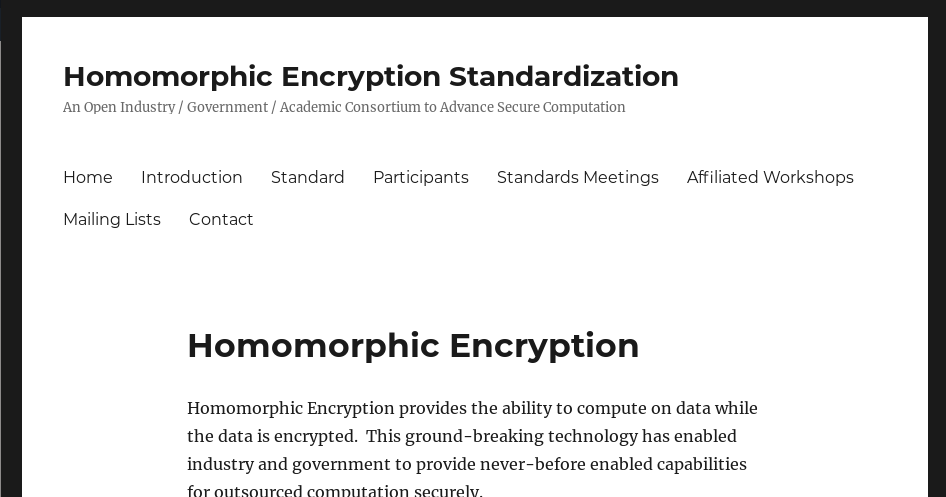
\includegraphics[width=\textwidth]{he-standard}
    \end{figure}
    \centering\url{https://homomorphicencryption.org/}

\end{frame}

\begin{frame}{Homomorphic Encryption Standarization}

    Estándar definido principalmente por tres elementos:
    
    \begin{itemize}
        \item API
        \item Seguridad de los esquemas
        \item Aplicaciones de la HE
    \end{itemize}{}
    
    Además de mantener encuentros de trabajo:
    
    \begin{itemize}
        \item Identifican librerías
        \item Generaciones de HE
    \end{itemize}

\end{frame}

\begin{frame}{Objetivos}
    Determinar viabilidad de implementaciones HE para sistemas en producción, en función de:
    \begin{itemize}
        \item Usabilidad
        
        ¿Es fácil de usar?
        
        \item Capacidad
        
        ¿Qué puede hacer?
        
        \item Eficiencia
        
        ¿Qué coste (computacional, económico...) tiene?
        
    \end{itemize}
\end{frame}


\section{Base teórica}

\begin{frame}{Lattice based cryptography}

    La seguridad de los sistemas criptográficos se basa en problemas matemáticos:
    
    \begin{itemize}
        \item Factorización
        \item Logaritmo discreto
        \item \textbf{Problemas con vectores} $\implies$ \textit{Lattice based crypto}
    \end{itemize}

    \begin{figure}
        \centering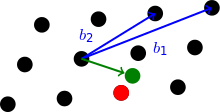
\includegraphics[width=0.5\textwidth]{cvp}
    \end{figure}

\end{frame}

\begin{frame}{LWE}

    Regev (\cite{regev_learning_2010}) propone un esquema criptográfico para el problema del aprendizaje con errores (\textbf{LWE})
    
    \begin{alertblock}{No solo HE}
    Los esquemas criptográficos basados en \textit{lattices} se postulan como sistemas \textit{post-quantum}
    \end{alertblock}

    \begin{figure}
        \centering
        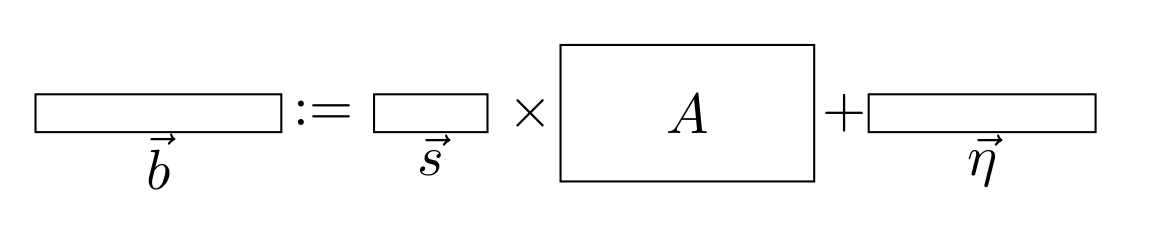
\includegraphics[width=\textwidth]{lwe}
    \end{figure}
    

\end{frame}


\begin{frame}{LWE}

    \begin{block}{Cifrado}
        \begin{enumerate}
            \item Generar valores $ a_i $ y $ b_i = (a_i \times s + e_i) \Mod{q} $
            \item Cifrar $ x $: $ (c1, c2) = (\sum_{j=1}^{m} a_{ij}, \sum_{j=1}^{m} b_{ij} + x * (q/2)) $
        \end{enumerate}
    \end{block}

    \begin{block}{Descifrado}
        \begin{enumerate}
            \item Descifrar $x$: $ x \approx c_2 - (c_1*s) $
            \begin{enumerate}
                \item $ b + x*(q/2) - a*s $
                \item $ a*s + e + x*(q/2) - a*s $
                \item $ e + x*(q/2) \approx x * (q/2) $
            \end{enumerate}
            \item Determinar el resultado
            \begin{enumerate}
                \item $x/(q/2) \approx 0 \implies x=0$
                \item $x/(q/2) \approx 1 \implies x=1$
            \end{enumerate}
        \end{enumerate}
    \end{block}
    
\end{frame}

\begin{frame}{LWE}

    \href{https://asciinema.org/a/qMaeVWh1ktPG9TULjmve7QzNT}{
        \centering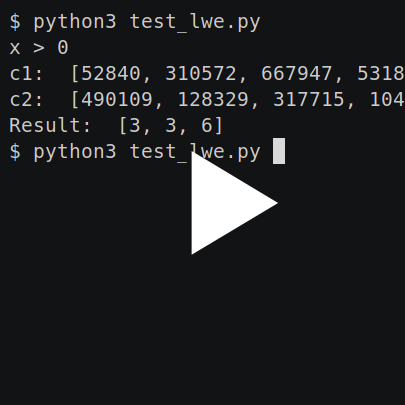
\includegraphics[width=0.5\textwidth]{test_lwe}
    }
    \centering\url{https://asciinema.org/a/qMaeVWh1ktPG9TULjmve7QzNT}

\end{frame}

\begin{frame}{Generaciones HE}
    
    Podemos diferenciar tres tipos de HE:
    
    \begin{itemize}
        \item Partially Homomorphic Encryption
        \item Somewhat Homomorphic Encryption (SHE)
        \item Fully Homormorphic Encryption (FHE)
    \end{itemize}
    
    Y tres generaciones (y pico) de HE:
    
    \begin{itemize}
        \item Pre-HE: RSA, Boneh–Goh–Nissim
        \item Primera generación: Técnica de \textit{bootstrapping} (\cite{gentry_fully_2009})
        \item Segunda generación: BGV, BFV, CKKS...
        \item Tercera generación: GSW, TFHE...
    \end{itemize}
 
\end{frame}

\section{Librerías}

\begin{frame}{Librerías del estándar}
    \begin{itemize}
        \item Segunda generación
        \begin{itemize}
            \item HELib
            \item \textbf{Microsoft SEAL}
            \item PALISADE
            \item HeaAn
            \item LoL
            \item NFLlib
        \end{itemize}
        \item Tercera generación
        \begin{itemize}
            \item \textbf{TFHE}
            \item FHEW
        \end{itemize}
    \end{itemize}
    
    \begin{alertblock}{Otras dos importantes (para futuro)}    
        \begin{itemize}
            \item cuHe (\url{https://github.com/vernamlab/cuHE})
            \item Cingulata (\url{https://github.com/CEA-LIST/Cingulata})
        \end{itemize}
    \end{alertblock}

\end{frame}

\begin{frame}{Microsoft SEAL}

    \begin{figure}[H]
        \centering
\includegraphics[width=0.5\textwidth]{logo_seal}
    \end{figure}
    \centering {
        \url{https://github.com/Microsoft/SEAL} \\ (\cite{noauthor_microsoft_2019})
    }
    
\end{frame}

\begin{frame}{Microsoft SEAL}

    \begin{itemize}
        \item Pocas operaciones
        
        Sumas, restas y productos.
        
        \item Capacidad limitada de cómputo
        
        Esquemas de segunda generación SHE (BFV y CKKS)

        \item Muy buena documentación

    \end{itemize}{}
    
\end{frame}

\begin{frame}{TFHE}

    \begin{figure}[H]
        \centering
\includegraphics[width=0.5\textwidth]{logo_tfhe}
    \end{figure}
    \centering{
        \url{https://github.com/tfhe/tfhe} \\ (\cite{chillotti_tfhe:_2016})
    }

\end{frame}

\begin{frame}{TFHE}

    \begin{itemize}
        \item Un esquema: TFHE
        \item Un parámetro: $\lambda$
        \item Sólo puertas lógicas
        \begin{itemize}
            \item OR, AND, XOR...
            \item NOT
            \item ¡MUX!
        \end{itemize}
        \item Cada puerta tarda $\sim20$ms
    \end{itemize}{}
    
    \begin{exampleblock}{}
      {\large ``Si Spiderman puede balancearse sobre su cuerda el tiempo suficiente para lanzar una nueva cuerda, ¡puede volar!''}
      \vskip5mm
      \hspace*\fill{\small--- El equipo de TFHE}
    \end{exampleblock}
\end{frame}

\section{Implementación}

\begin{frame}{Geoposicionamiento}

    \begin{figure}[H]
        \begin{overprint}
            \onslide<1>\centering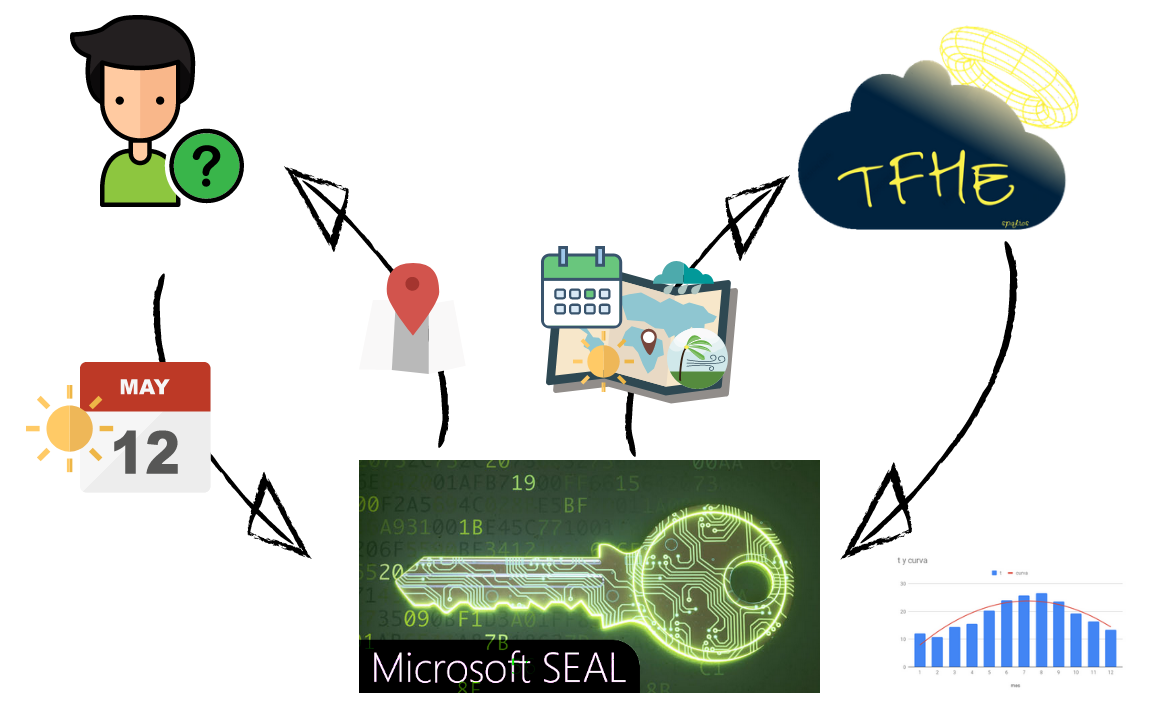
\includegraphics[width=\textwidth]{sistema_completo}
            \onslide<2>\centering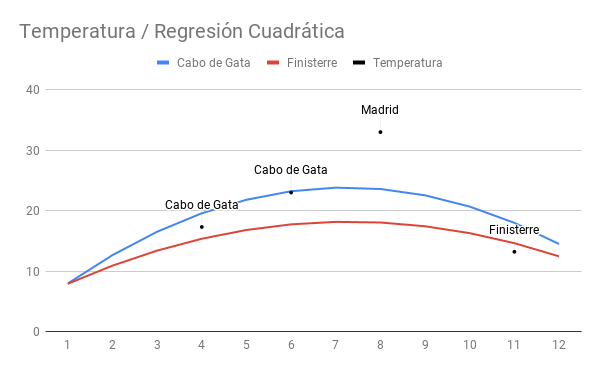
\includegraphics[width=\textwidth]{t_vs_r2}
        \end{overprint}
    \end{figure}

\end{frame}

\begin{frame}{TFHE}
    \begin{itemize}
        \item Generar curva de regresión
        
        \begin{figure}[H]
            \centering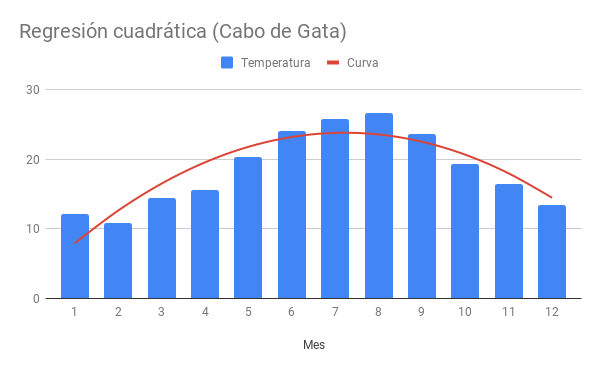
\includegraphics[width=0.85\textwidth]{reg2_cg}
        \end{figure}
    \end{itemize}
\end{frame}

\begin{frame}{Curva de regresión}

    \begin{block}{Fórmula de curva}
        \vspace*{-\baselineskip}\setlength\belowdisplayshortskip{0pt}
        \begin{align*}
        y = ax^2 + bx + c
        \end{align*}
    \end{block}
    
    \begin{block}{Parametrización de curva}
        \vspace*{-\baselineskip}\setlength\belowdisplayshortskip{0pt}
        \begin{align*}
            \begin{cases}
                \sum_{i=0}^n y_i         &= a*\sum_{i=0}^n x_i^2 + b*\sum_{i=0}^n x_i   + c*n \\
                \sum_{i=0}^n x_i * y_i   &= a*\sum_{i=0}^n x_i^3 + b*\sum_{i=0}^n x_i^2 + c*\sum_{i=0}^n x_i \\
                \sum_{i=0}^n x_i^2 * y_i &= a*\sum_{i=0}^n x_i^4 + b*\sum_{i=0}^n x_i^3 + c*\sum_{i=0}^n x_i^2
            \end{cases}
        \end{align*}
    \end{block}
    \begin{alertblock}{¿Qué necesitamos?}
    Sólo necesitamos saber $a$, $b$ y $c$ para reconstruir la curva
    \end{alertblock}
\end{frame}


\begin{frame}{tfhe-math}

    \begin{figure}[H]
        \centering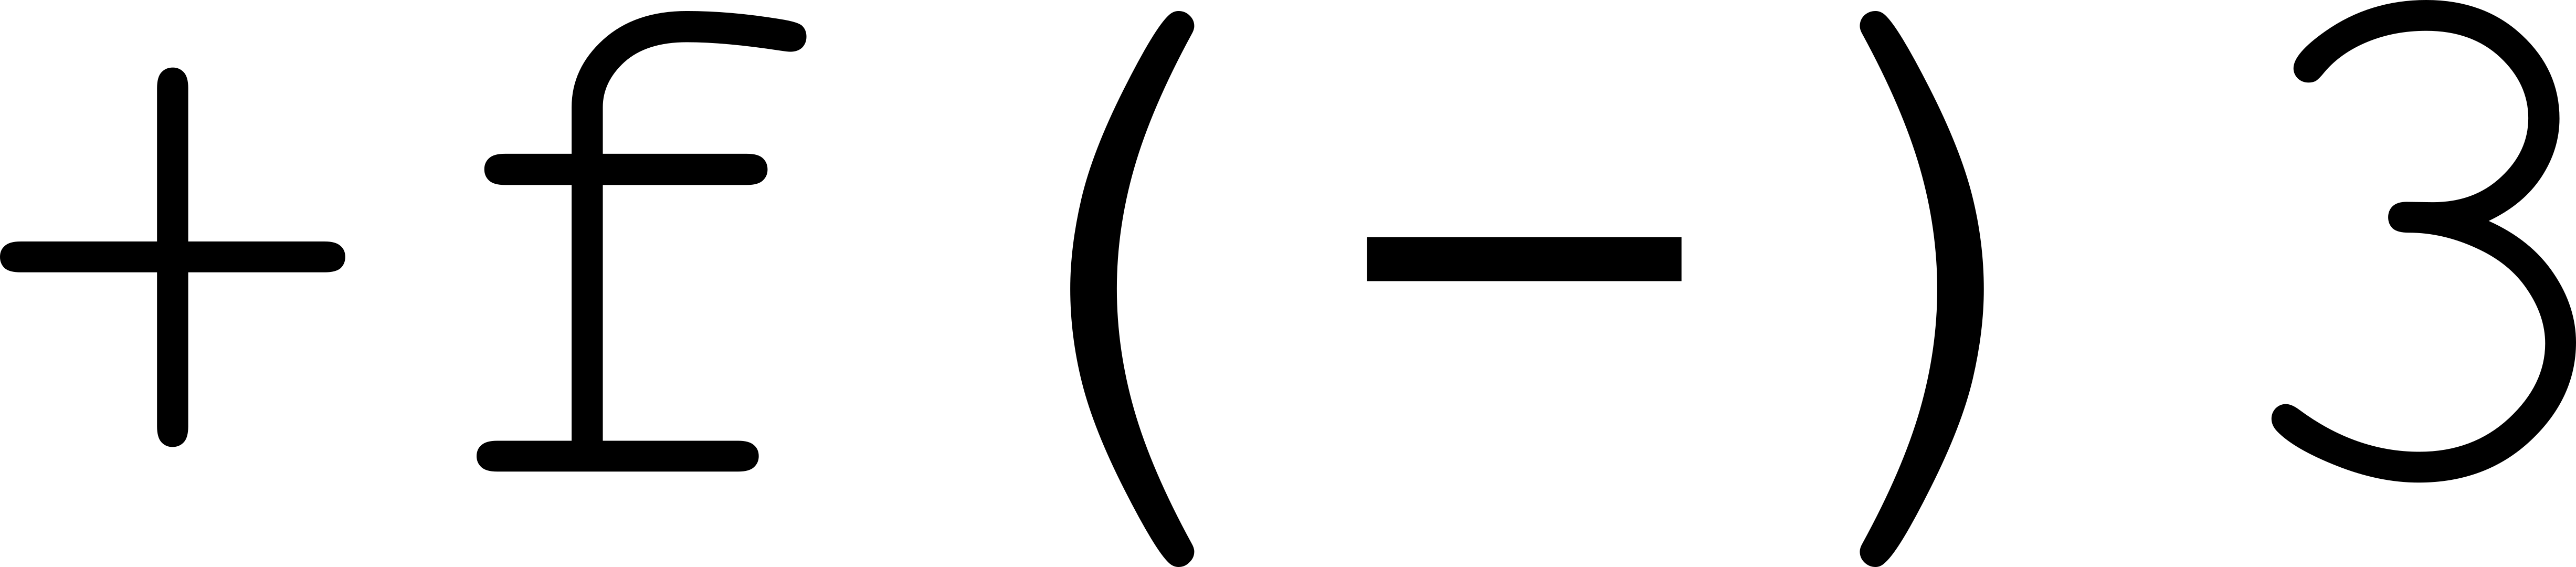
\includegraphics[width=0.5\textwidth]{logo-tfhe-math}
    \end{figure}
    \centering{
        \url{https://gitlab.com/junquera/tfhe-math} \\ (\cite{junquera_tfhe_2019})
    }
\end{frame}


\begin{frame}{tfhe-math}
    \begin{itemize}
        
        \item Operaciones aritméticas con puertas lógicas ($+$, $-$, $*$, $\div$)
        
        \begin{figure}[H]
            \centering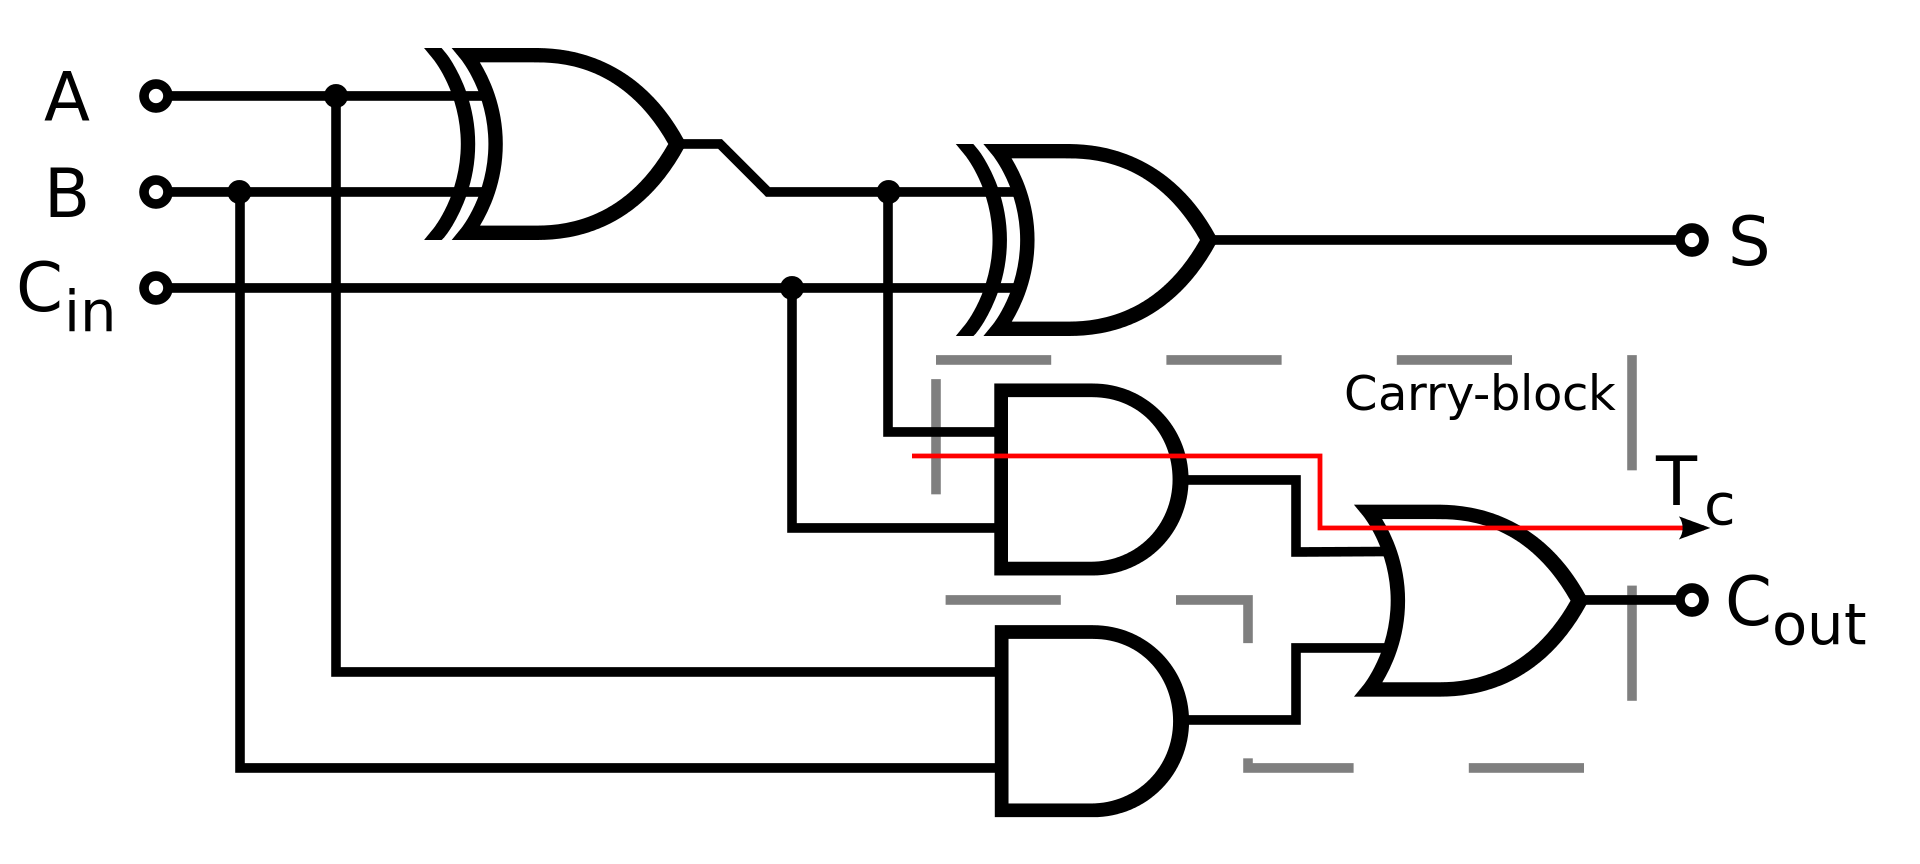
\includegraphics[width=0.75\textwidth]{adder_digital_circuit}
        \end{figure}
        
        \item Gestión de signo, decimales y tamaño de palabra
        
    \end{itemize}
\end{frame}

\begin{frame}{Demo TFHE}

    \href{https://asciinema.org/a/4S69lCdKI25Q6ALYzcqNTTIEa}{
        \centering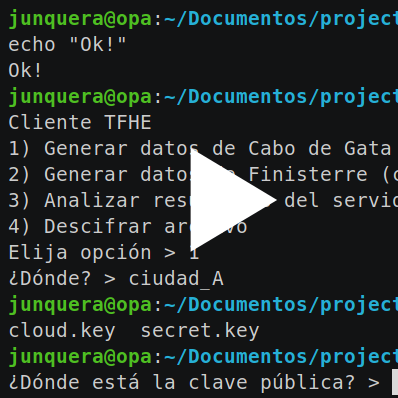
\includegraphics[width=0.5\textwidth]{tfhe-cs}
    }
    \centering\url{https://asciinema.org/a/4S69lCdKI25Q6ALYzcqNTTIEa}

\end{frame}

\begin{frame}{SEAL}
    \begin{itemize}
        \item Distancia de punto a curvas (CKKS + \textit{Batching})
        \begin{align*}
        \begin{pmatrix}
            d_1 \\
            d_2 \\
            \vdots{} \\
            d_n
        \end{pmatrix}
        =
        y - (x^2 *
        \begin{pmatrix}
            a_1 \\
            a_2 \\
            \vdots{} \\
            a_n
        \end{pmatrix}
        + x *
        \begin{pmatrix}
            b_1 \\
            b_2 \\
            \vdots{} \\
            b_n
        \end{pmatrix}
        +
        \begin{pmatrix}
            c_1 \\
            c_2 \\
            \vdots{} \\
            c_n
        \end{pmatrix}
        )
        \label{form:distancias_seal}
    \end{align*}
    \end{itemize}{}
\end{frame}

\begin{frame}{Demo SEAL}

    \href{https://asciinema.org/a/5OTphARYxFoRAkfahycjjTsSA}{
        \centering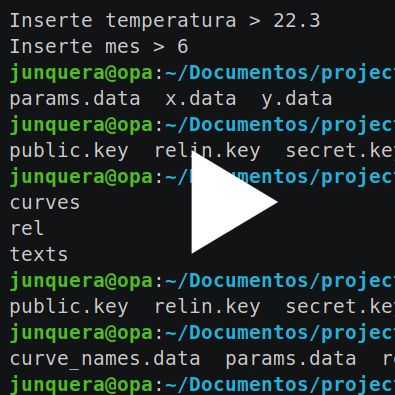
\includegraphics[width=0.5\textwidth]{seal-cs}
    }
    \centering\url{https://asciinema.org/a/5OTphARYxFoRAkfahycjjTsSA}

\end{frame}


\section{Resultados}

\begin{frame}{Resultados TFHE}
    \begin{table}[]
        \centering
        \begin{tabular}{ r | ccc }
            operación       & puertas lógicas       & tiempo estimado & tiempo real \\
            \hline \hline
            compare\_bit     & 2     & 0,04 & 0 \\
            equal   & 128   & 2,56  & 3 \\
            is\_negative     & 1     & 0,02 & 0 \\
            minimum/maximum & 388   & 7,76  & 14  \\
            add\_bit    & 5     & 0,1  & 0 \\
            sum     & 320   & 6,4 & 8 \\
            negativo        & 192   & 3,84  & 8 \\
            resta   & 512   & 10,24 & 16  \\
            multiply        & 46826 & 936,52  & 1257  \\
            mayor\_igual     & 128   & 2,56 & 4 \\
            shiftl/shiftr   & 771   & 15,42 & 19  \\
            u\_shiftl/u\_shiftr       & 129   & 2,58  & 0 \\
            divide  & 85776 & 1715,52 & 11662
        \end{tabular}
    \end{table}
\end{frame}

\begin{frame}{Crecimiento TFHE}
    \begin{figure}[H]
        \centering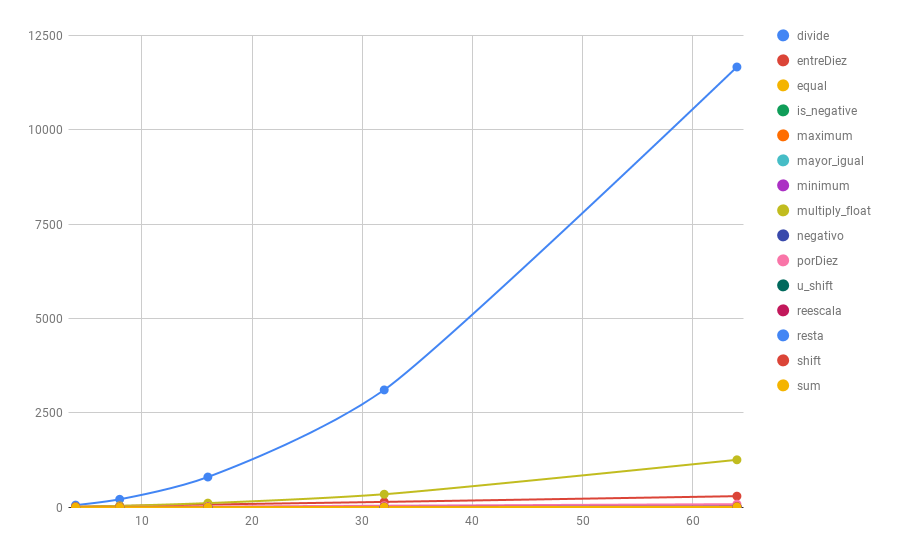
\includegraphics[width=\textwidth]{crec_func}
    \end{figure}
\end{frame}

\begin{frame}{Tiempo cálculo de curva}
    \begin{table}[]
        \centering
        \begin{tabular}{r | c c c c}
            Cálculo & Tiempo estimado (s) & Tiempo real (s) & Proporción \\
            \hline \hline
            initVectores  & 76092 & 68940  & 0.90 \\
            calcCuadrados & 5028  & 4555 & 0.90 \\
            calcDuplas  & 11313 & 10431 & 0.92 \\
            calcComplejos & 12570 & 11522 & 0.91 \\
            CalcC & 46776 & 39818  & 0.85 \\
            CalcB & 14208 & 12222  & 0.86 \\
            CalcA & 14192 & 12200  & 0.86 \\
            Total & 180179  & 159688 & 0.89 \\
            \hline
            &  & \textbf{¡1.84d!} & \\
        \end{tabular}
    \end{table}
    % TODO ASCIINEMA reg2py
\end{frame}

\begin{frame}{Resultados SEAL}

    \begin{alertblock}{Muy rápida pero...}
        \begin{itemize}
            \item Máximo 19 multiplicaciones realizables teóricamente
            \item Trabajar con números pequeños (en la práctica, menos de 9 productos, o rompe el esquema)
        \end{itemize}
    \end{alertblock}

\end{frame}

\begin{frame}{Costes de desarrollo}

    \begin{table}[]
        \centering
        \begin{tabular}{| r | l c | }
            \hline
            \textbf{Estudio teórico} & 2 meses, 2 horas semana   & $\implies$ 18 horas \\
            \hline
            \textbf{Estudiar libs.} & 1,5 meses, 2 horas semana &  $\implies$ 12 horas \\
            \hline
            \textbf{Implementación} & 1 mes, 6 horas día     & $\implies$ 90 horas \\
            \hline
        \end{tabular}
    \end{table}
    
    \begin{block}{Coste total}
        \centering{
            Con un sueldo mínimo de $30000\euro/$año\footnote{Cuánto gana un ingeniero informático, \url{https://universidadeuropea.es/blog/cuanto-gana-un-ingeniero-informatico}}:
        }
        \vspace*{-5pt}\setlength\belowdisplayshortskip{15pt}
        \begin{align*}
        120 horas * 15 \euro/hora = 1800 \euro  
        \end{align*}
    \end{block}{}

\end{frame}


\begin{frame}{Costes de despliegue}

    \begin{figure}[H]
        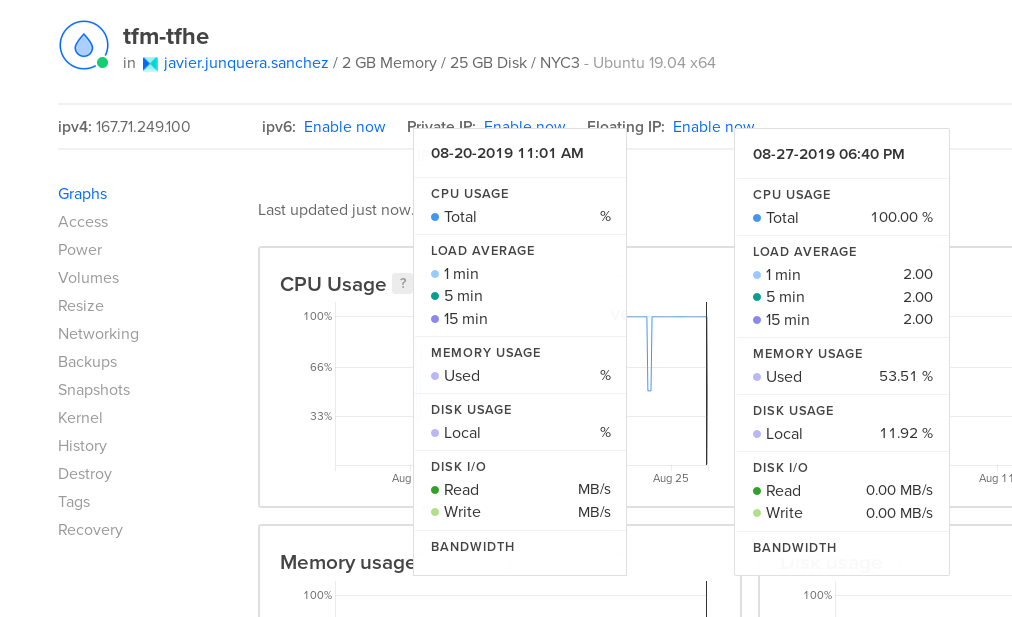
\includegraphics[width=\textwidth]{stats-do}
    \end{figure}
    
\end{frame}

\begin{frame}{Costes de despliegue}

    \begin{block}{Ejecución en cloud}
        Una semana en Digital Ocean\footnote{\url{https://www.digitalocean.com/}}:
        \begin{itemize}
            \item Un día, un núcleo de CPU:     a $5\$/$mes
            \item 6 días, 2 CPUs (al $100\%$):  a $15\$/$mes
        \end{itemize}
        El coste final ha sido de $5,07\$$ ($\sim4,6$\euro)
    \end{block}   
    
\end{frame}

\section{Conclusiones}


\begin{frame}{Conclusiones}
    \begin{itemize}
        \item Medidas basadas en riesgo
        \begin{figure}[H]
            \centering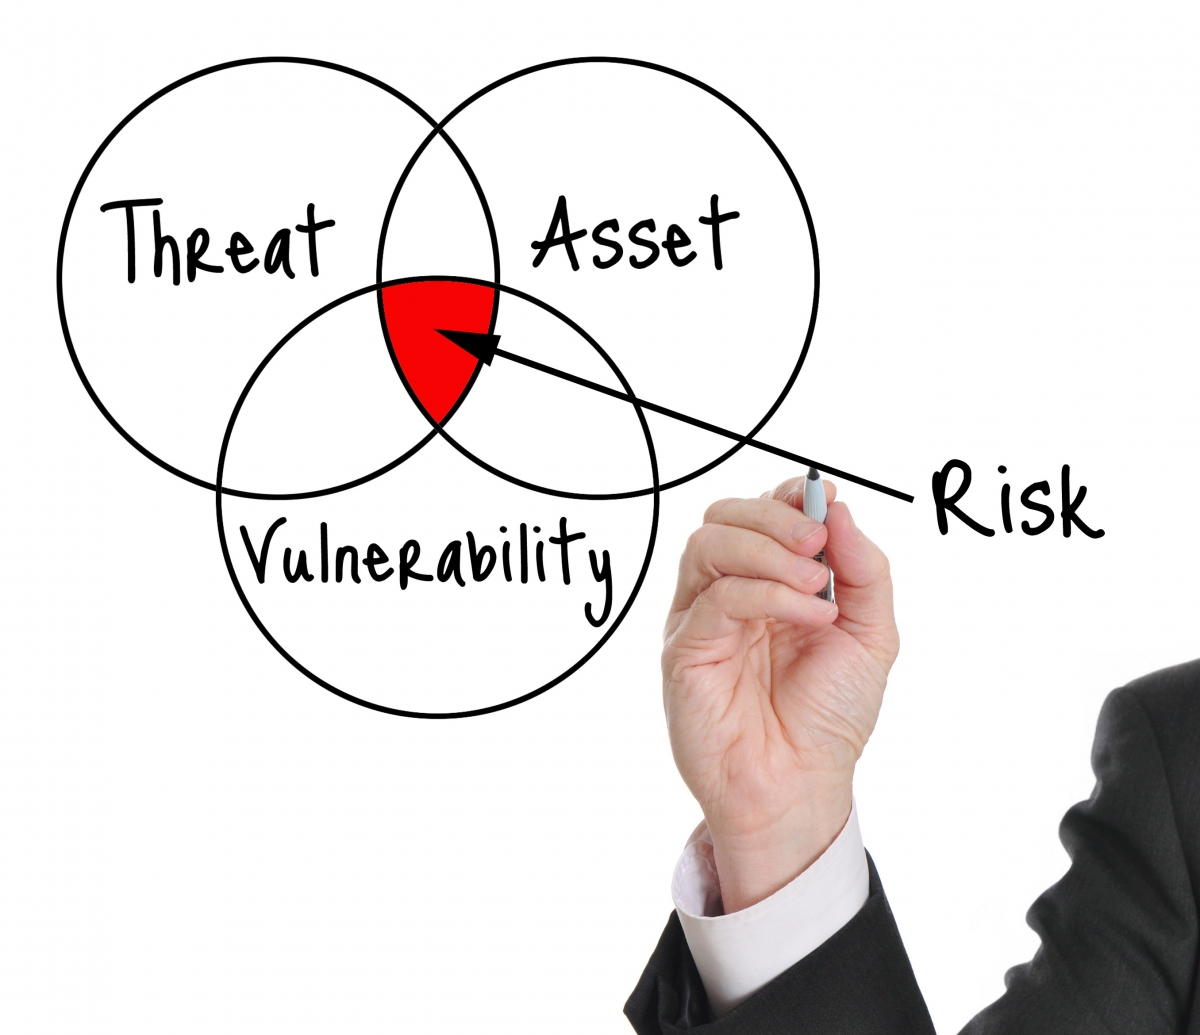
\includegraphics[width=0.5\textwidth]{arr}
        \end{figure}
    \end{itemize}
\end{frame}

\begin{frame}{Conclusiones}
    \begin{itemize}
        \item Solucionar problemas irresolubles sin HE, no problemas ya resueltos
        \begin{figure}[H]
            \centering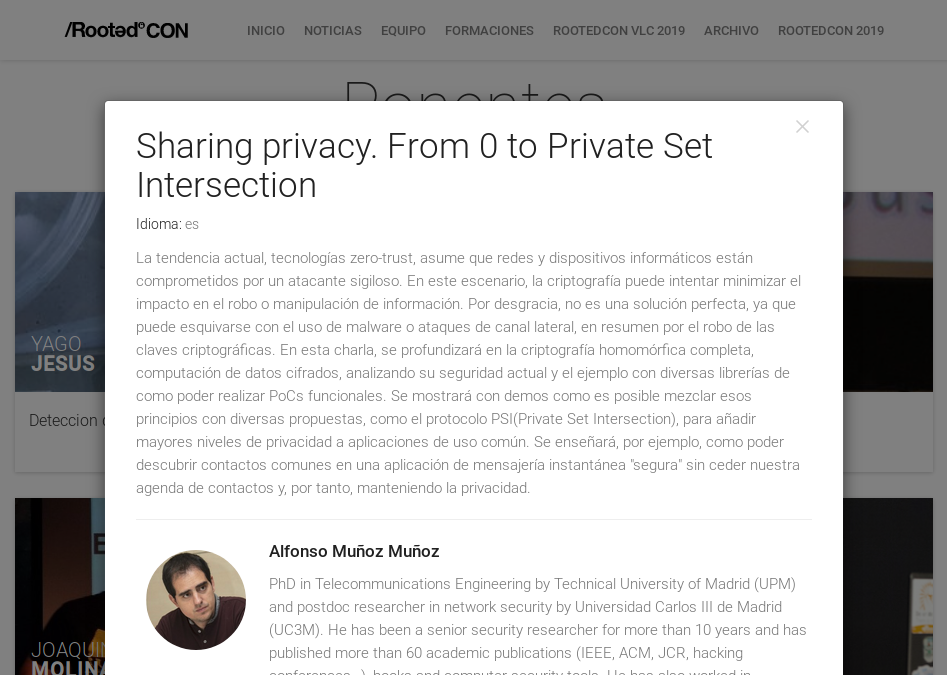
\includegraphics[width=0.75\textwidth]{psi-alfonso}
        \end{figure}
    \end{itemize}
\end{frame}

\begin{frame}{Conclusiones}
    \begin{itemize}
        \item Actualmente, cualquier implementación tiene que ser ``bajo supervisión''
        \begin{figure}[H]
            \centering
\includegraphics[width=0.5\textwidth]{low-sec}
        \end{figure}
    \end{itemize}
\end{frame}

\begin{frame}{Conclusiones}
    \begin{itemize}
        \item Hacer implementaciones a medida
        \begin{figure}[H]
            \centering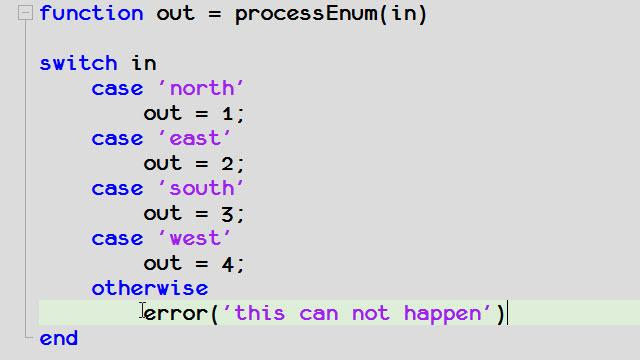
\includegraphics[width=0.75\textwidth]{simple-logic}
        \end{figure}
    \end{itemize}
\end{frame}

\begin{frame}{Conclusiones}
    \begin{itemize}
        \item Hacer implementaciones \textbf{a medida}
        \begin{figure}[H]
            \centering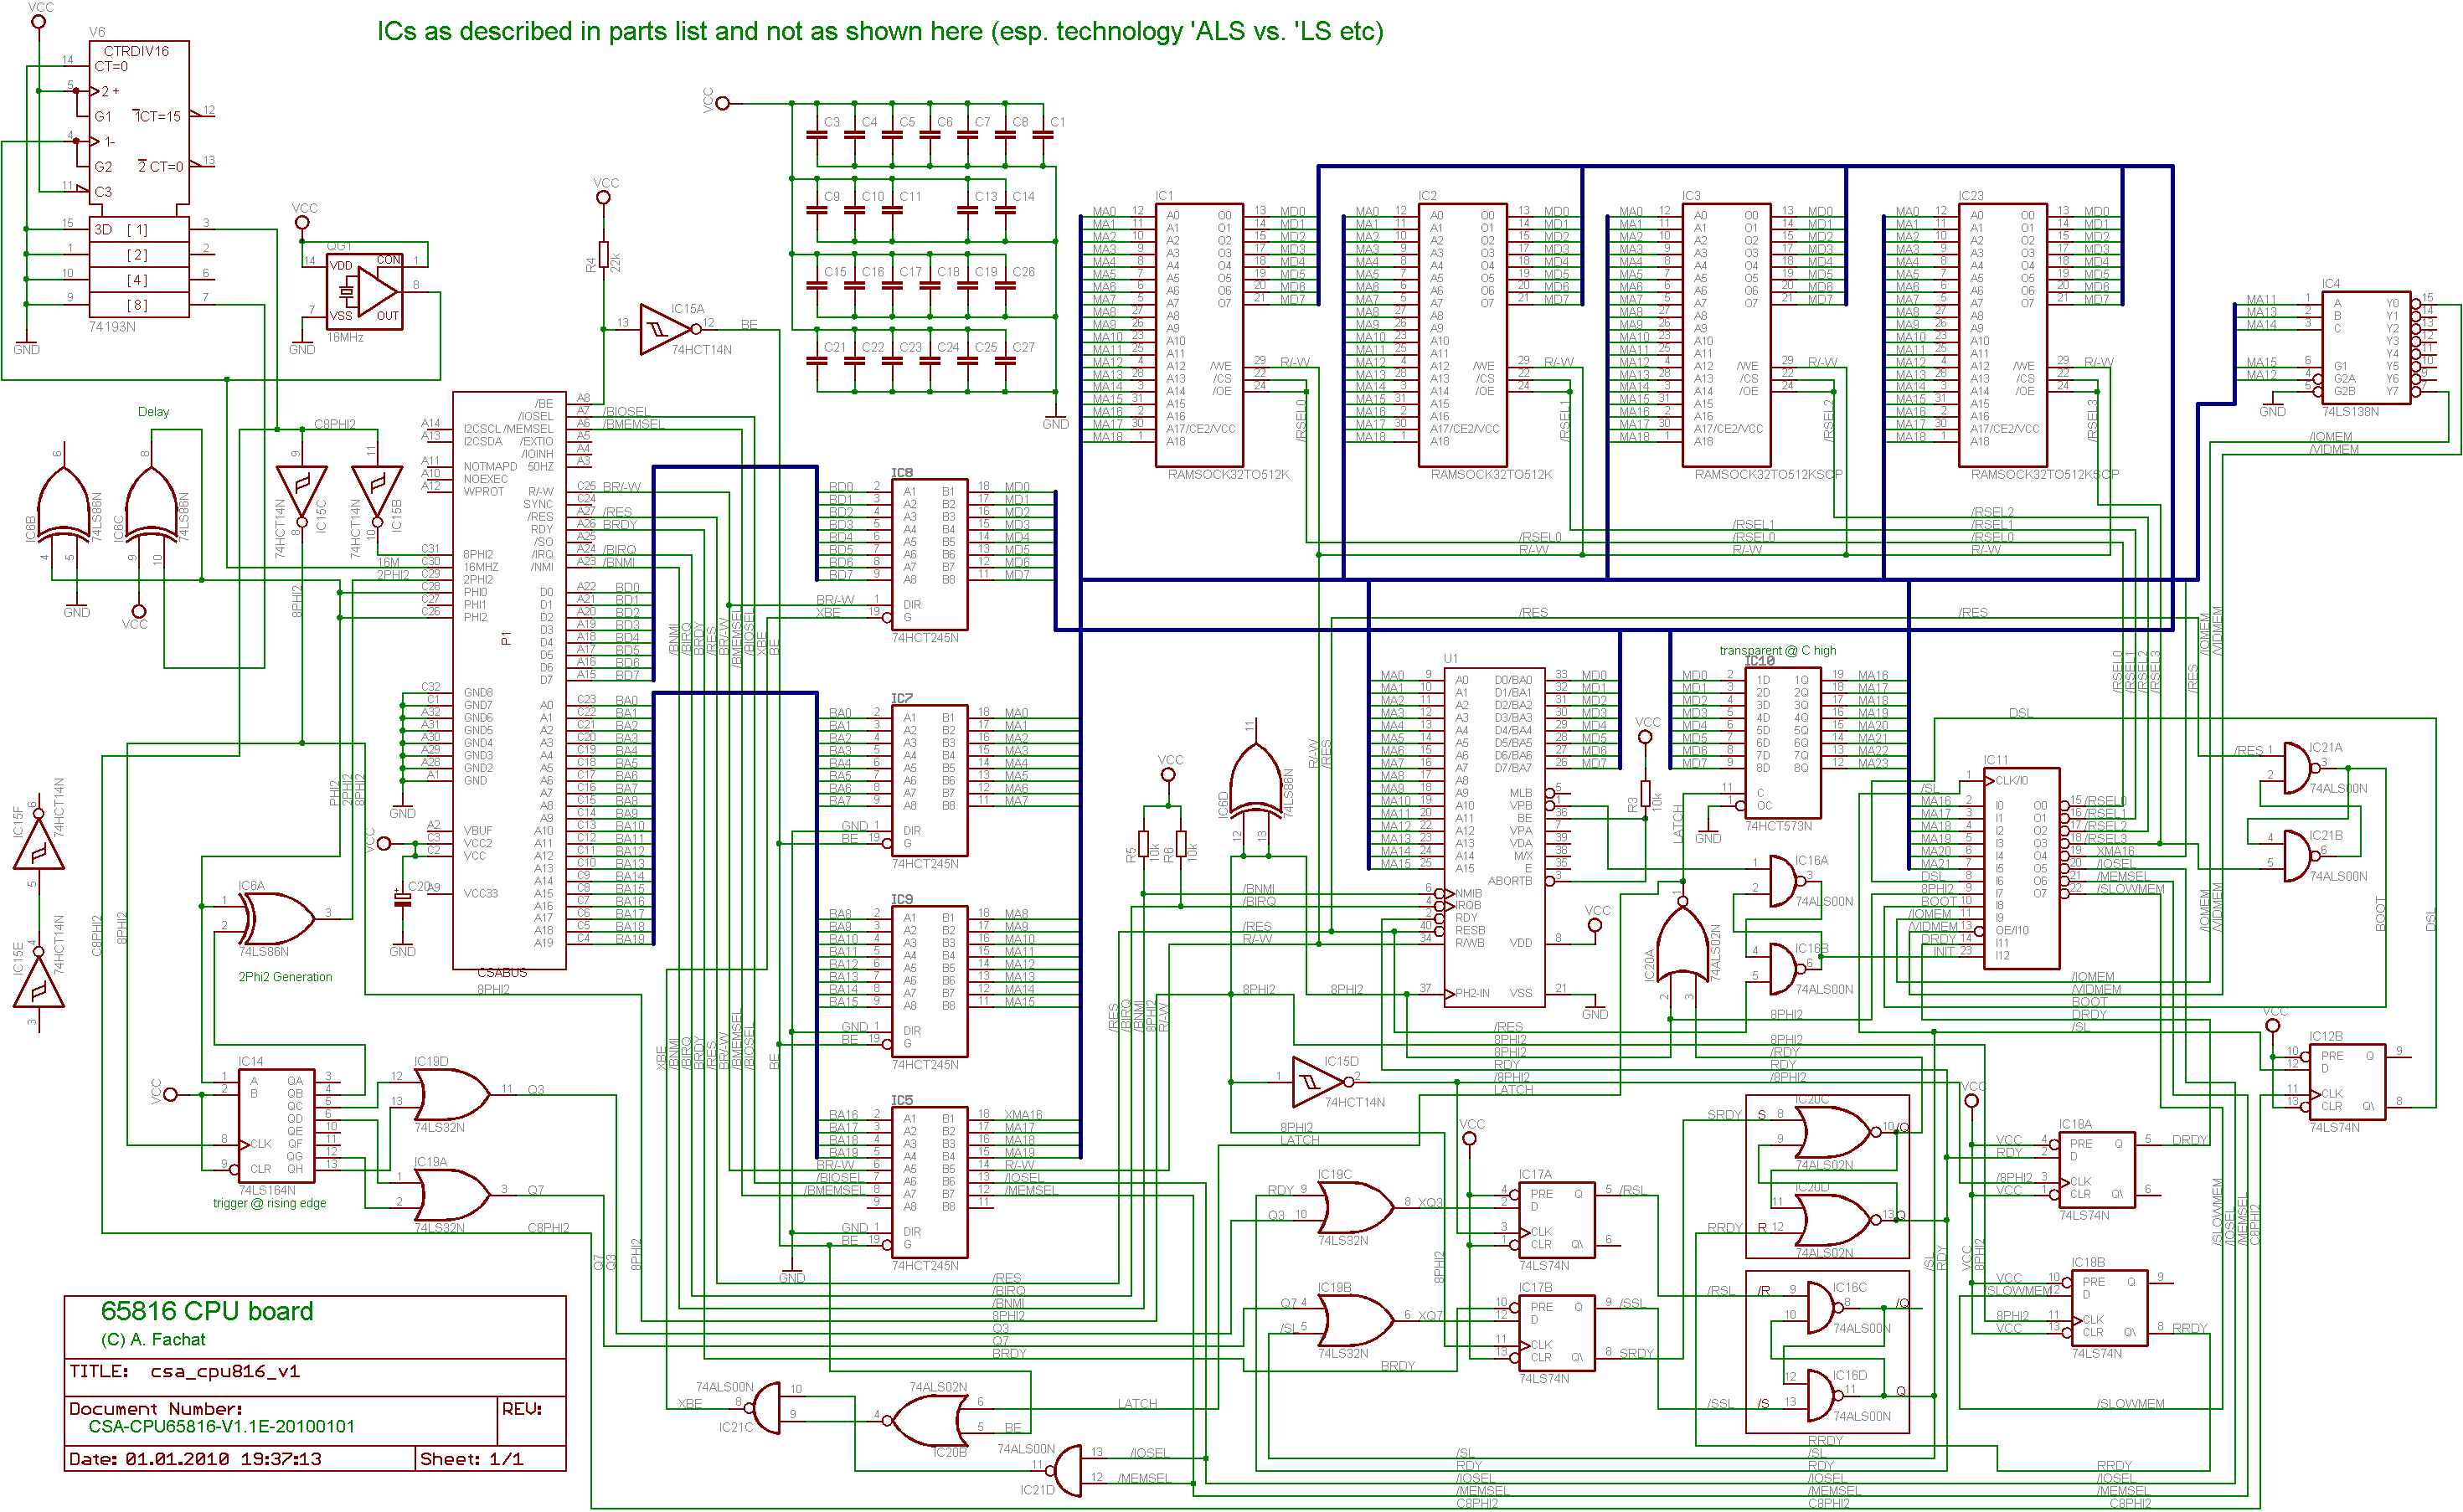
\includegraphics[width=0.75\textwidth]{complex-logic}
        \end{figure}
    \end{itemize}
\end{frame}

\section{Trabajos futuros}

\begin{frame}{Trabajos futuros}

    \begin{itemize}
        \item \texttt{cuHE}\footnote{\url{https://github.com/vernamlab/cuHE}}
        
        Paralelización con GPU
        
        \item Cingulata\footnote{\url{https://github.com/CEA-LIST/Cingulata}} + ABY\footnote{\url{https://github.com/encryptogroup/ABY}}
        
        Compilador de \texttt{C++} a código HE \& Repositorio con circuitos lógicos
        
        \vspace{15pt}
        
        \begin{figure}[H]
            \adjustimage{width=0.7\textwidth,right}{cingulata}
        \end{figure}
        
    \end{itemize}

\end{frame}

\section*{Fin}

\begin{frame}
    \frametitle{Bibliografía}
    \printbibliography
\end{frame}

\begin{frame}{¡Gracias!}

    \centering\large No es difícil de procesar... \\
    \vspace*{15pt}
    \centering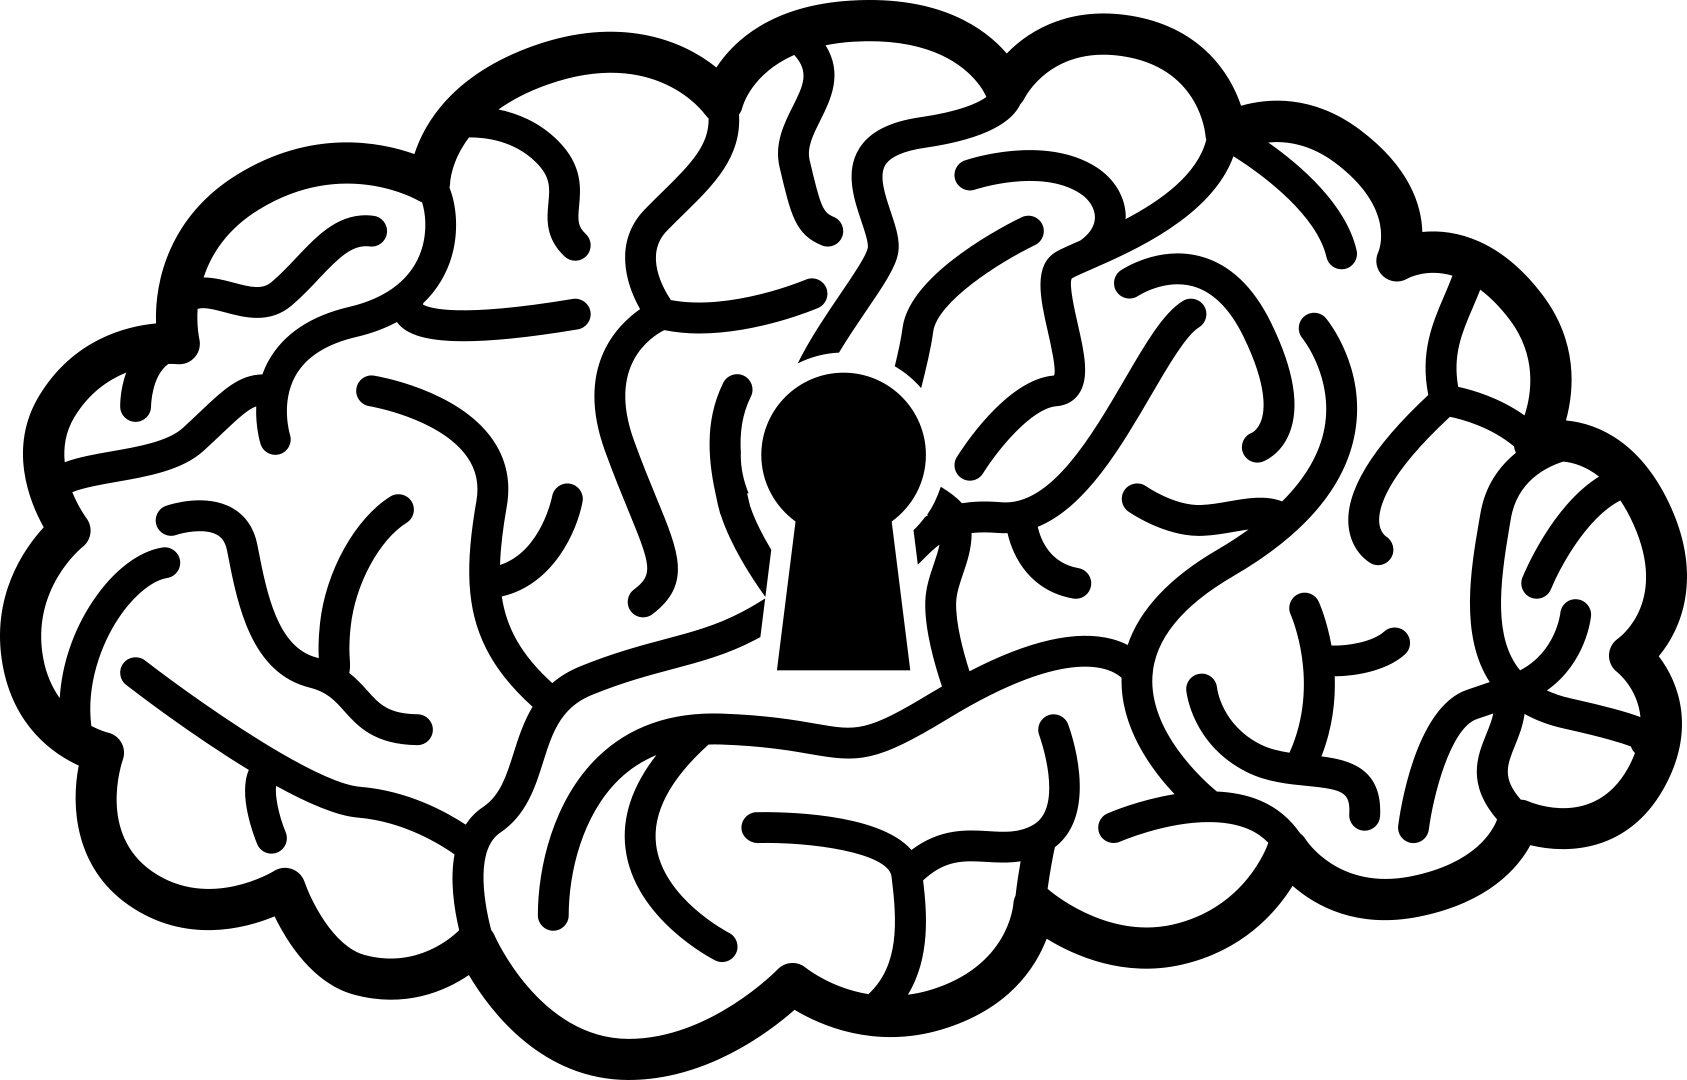
\includegraphics[width=0.35\textwidth]{mindcrypt} \\
    \vspace{10pt}
    \centering\huge ¡Es que está cifrado!

\end{frame}


\end{document}

% \begin{frame}
% \frametitle{Blocks of Highlighted Text}
% \begin{block}{Block 1}
% Lorem ipsum dolor sit amet, consectetur adipiscing elit. Integer lectus nisl, ultricies in feugiat rutrum, porttitor sit amet augue. Aliquam ut tortor mauris. Sed volutpat ante purus, quis accumsan dolor.
% \end{block}

% \begin{block}{Block 2}
% Pellentesque sed tellus purus. Class aptent taciti sociosqu ad litora torquent per conubia nostra, per inceptos himenaeos. Vestibulum quis magna at risus dictum tempor eu vitae velit.
% \end{block}

% \begin{block}{Block 3}
% Suspendisse tincidunt sagittis gravida. Curabitur condimentum, enim sed venenatis rutrum, ipsum neque consectetur orci, sed blandit justo nisi ac lacus.
% \end{block}
% \end{frame}

% %------------------------------------------------

% \begin{frame}
% \frametitle{Multiple Columns}
% \begin{columns}[c] % The "c" option specifies centered vertical alignment while the "t" option is used for top vertical alignment

% \column{.45\textwidth} % Left column and width
% \textbf{Heading}
% \begin{enumerate}
% \item Statement
% \item Explanation
% \item Example
% \end{enumerate}

% \column{.5\textwidth} % Right column and width
% Lorem ipsum dolor sit amet, consectetur adipiscing elit. Integer lectus nisl, ultricies in feugiat rutrum, porttitor sit amet augue. Aliquam ut tortor mauris. Sed volutpat ante purus, quis accumsan dolor.

% \end{columns}
% \end{frame}

% %------------------------------------------------
% \section{Second Section}
% %------------------------------------------------

% \begin{frame}
% \frametitle{Table}
% \begin{table}
% \begin{tabular}{l l l}
% \toprule
% \textbf{Treatments} & \textbf{Response 1} & \textbf{Response 2}\\
% \midrule
% Treatment 1 & 0.0003262 & 0.562 \\
% Treatment 2 & 0.0015681 & 0.910 \\
% Treatment 3 & 0.0009271 & 0.296 \\
% \bottomrule
% \end{tabular}
% \caption{Table caption}
% \end{table}
% \end{frame}

% %------------------------------------------------


